%%
%% This is file `sample-sigchi.tex',
%% generated with the docstrip utility.
%%
%% The original source files were:
%%
%% samples.dtx  (with options: `sigchi')
%% 
%% IMPORTANT NOTICE:
%% 
%% For the copyright see the source file.
%% 
%% Any modified versions of this file must be renamed
%% with new filenames distinct from sample-sigchi.tex.
%% 
%% For distribution of the original source see the terms
%% for copying and modification in the file samples.dtx.
%% 
%% This generated file may be distributed as long as the
%% original source files, as listed above, are part of the
%% same distribution. (The sources need not necessarily be
%% in the same archive or directory.)
%%
%% The first command in your LaTeX source must be the \documentclass command.
\documentclass[sigchi]{acmart}

%%
%% \BibTeX command to typeset BibTeX logo in the docs

\AtBeginDocument{%
  \providecommand\BibTeX{{%
    \normalfont B\kern-0.5em{\scshape i\kern-0.25em b}\kern-0.8em\TeX}}}

%% Rights management information.  This information is sent to you
%% when you complete the rights form.  These commands have SAMPLE
%% values in them; it is your responsibility as an author to replace
%% the commands and values with those provided to you when you
%% complete the rights form.

%% These commands are for a PROCEEDINGS abstract or paper.
\acmConference[MLDM-M1]{DataMining Project Report}
\acmBooktitle{Online New Popularity}


%%
%% Submission ID.
%% Use this when submitting an article to a sponsored event. You'll
%% receive a unique submission ID from the organizers
%% of the event, and this ID should be used as the parameter to this command.
%%\acmSubmissionID{123-A56-BU3}

%%
%% The majority of ACM publications use numbered citations and
%% references.  The command \citestyle{authoryear} switches to the
%% "author year" style.
%%
%% If you are preparing content for an event
%% sponsored by ACM SIGGRAPH, you must use the "author year" style of
%% citations and references.
%% Uncommenting
%% the next command will enable that style.
%%\citestyle{acmauthoryear}

%%
%% end of the preamble, start of the body of the document source.
\setcopyright{none}
\setcopyright{none}
\begin{document}

%%
%% The "title" command has an optional parameter,
%% allowing the author to define a "short title" to be used in page headers.
\title{\\Insights of Online News Popularity Data Set\\ Data Mining Project Report}
%% used to denote shared contribution to the research.
\author{Yogesh KUMAR PILLI}
\author{ MLDM - M1 }
\email{yogesh.kumar@etu.univ-st-etienne.fr}
%\orcid{1234-5678-9012}
%\authornotemark[1]

\affiliation{%
  \institution{Université Jean Monnet}
  \streetaddress{10 Rue Tréfilerie }
  \city{Saint-Étienne}
  \state{Loire}
  \country{France}
  \postcode{42100}
}



%%
%% By default, the full list of authors will be used in the page
%% headers. Often, this list is too long, and will overlap
%% other information printed in the page headers. This command allows
%% the author to define a more concise list
%% of authors' names for this purpose.
\renewcommand{\shortauthors}{Yogesh Kumar Pilli}

%%
%% The abstract is a short summary of the work to be presented in the
%% article.
\begin{abstract}
  Over the past few decades Internet has drastically changed the way ideas, stories, facts are propagated across readership. We as a society have evolved technologically. Having said that, although it’s easier to publish articles online with little or no cost involved, yet finding the readers for it is an altogether different task. How and why does an article get popular is the real mystery.In this study, I have intend to use a dataset to identify the criteria that make articles popular. I have also intend to do a comparative study of various Data Mining algorithms on ‘Online News Popularity Dataset’ and see how they fair with each other in determining whether an article will be popular or not. 
\end{abstract}

%%
%% The code below is generated by the tool at http://dl.acm.org/ccs.cfm.
%% Please copy and paste the code instead of the example below.
%%
%%
%% Keywords. The author(s) should pick words that accurately describe
%% the work being presented. Separate the keywords with commas.
\keywords{Data Preprocessing,Regression,Classification,Machine Learning Algorithms}


%%
%% This command processes the author and affiliation and title
%% information and builds the first part of the formatted document.
\makeatletter
\def\@copyrightspace{\relax}
\makeatother
\maketitle

\section{Problem Understanding and Motivation}
Online articles are becoming more and more prominent, as they have already crowded out more tradition news outlets, and are continuing to expand. There are very few articles that go viral, but those select few that do, get a substantially larger number of shares and views than most other articles.More importantly, the demographic for viewers of online articles is dis-proportionally skewed towards teens and young adults, a prime target for many companies to run advertisement campaigns on social media\cite{SocialMedia}.As a well-known parameter, the number of shares determines the popularity of the news which in turn results in the revenue through advertisements. The key challenge in predicting the popularity of a blog post is it vastly depends on human behaviour as mentioned in the research “A survey on predicting the popularity of web content”\cite{SurveyPrediction}.
\section{Data Understanding}
The data source is from UCI Machine learning library\cite{UCIOnlineNewsData}. The well-known attributes such as the number of keywords, the category of the blog post was easily understandable. The major hindrance was on the initial understanding of the analytics information provided in the data set such as LDA, polarity, subjectivity which demanded more knowledge on the text mining techniques which was briefly inferred from “Large scale sentiment analysis for news and blogs”\cite{Large-Scale}. So, the variety in the data was also a critical factor in deciding the next steps.

Following features are of critical importance when understanding the data set::
\begin{itemize}
\item  It is a Multivariate data set as is evident from the Number of Attributes which is 61.
\item Attributes are all Integer or Real barring URL and time delta which are Non-Predictive in nature.
\item Total Number of Rows/Instance: 39797
\item  Total Number of Columns/Attributes: 61
\end{itemize}

 
\section{Data Preperation}
To be able to make sense of the data, all of data sets are engineered for features.
\subsection{Data Pre-Processing}
Processing of the data to plays a vital role in understanding the data as well as making the model more robust.The dataset was split into training and test sets, with an 70/30 ratio. All the 58 predictors and the response variable were analyzed for the detection of missing values, outliers and collinearity between predictors.Lets Study our data as stated below parameters
Does the subjects and Publishing days of news matters



\begin{figure}[h!]
  \caption{Distribution of share's with the different subject of news}
  \centering
  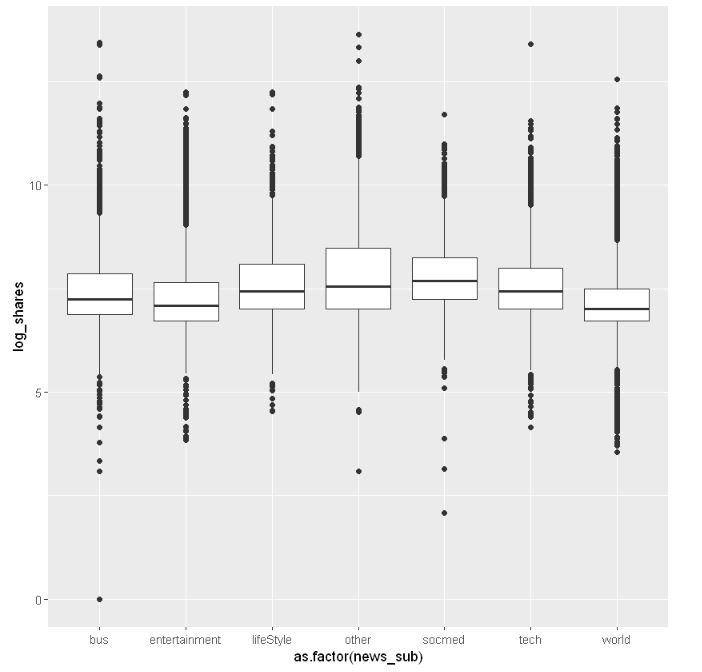
\includegraphics[width=0.5\textwidth]{SubjectofNews.JPG}
\end{figure}
From the Figure 1, You can see that all subjects looks similar regarding share numbers.


\begin{figure}[h!]
    \caption{Distribution of share's with different days in a week}
    \centering
    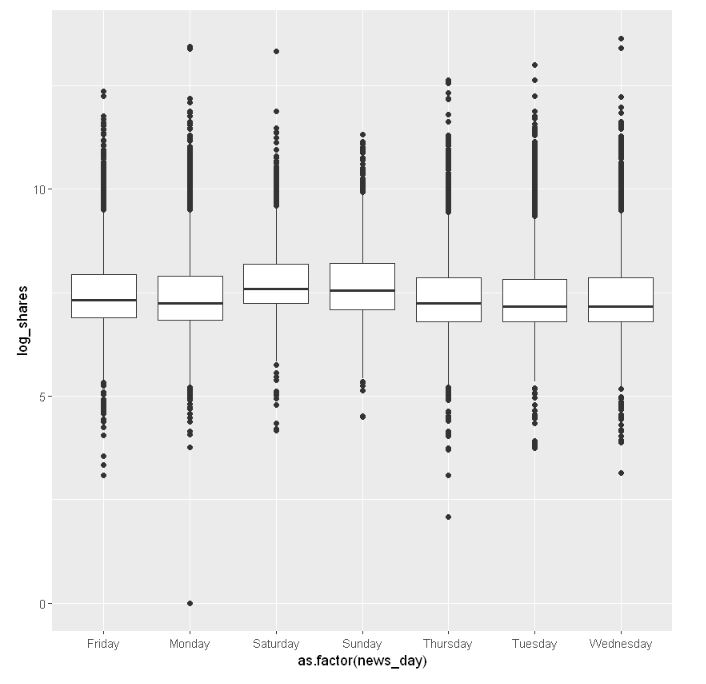
\includegraphics[width=0.5\textwidth]{Newsdays.JPG}
\end{figure}

Publishing day didn't show much influence on shares neither.In order make our data clear I have get ridden all the unwanted indicators. 


\subsection{Preprocessing through PCA}
A full feature set may include much noise. I had first attempted PCA for dimension reduction but it did not provide any improvements for our models,As PCA is a commonly used as dimensionality reduction algorithm\cite{Li}.However, the PCA results could only made our models perform worse. This is because the original feature set is well-designed and correlated information between features is limited.

\begin{figure}[h!]
    \caption{Principal component analysis on first two components}
    \centering
    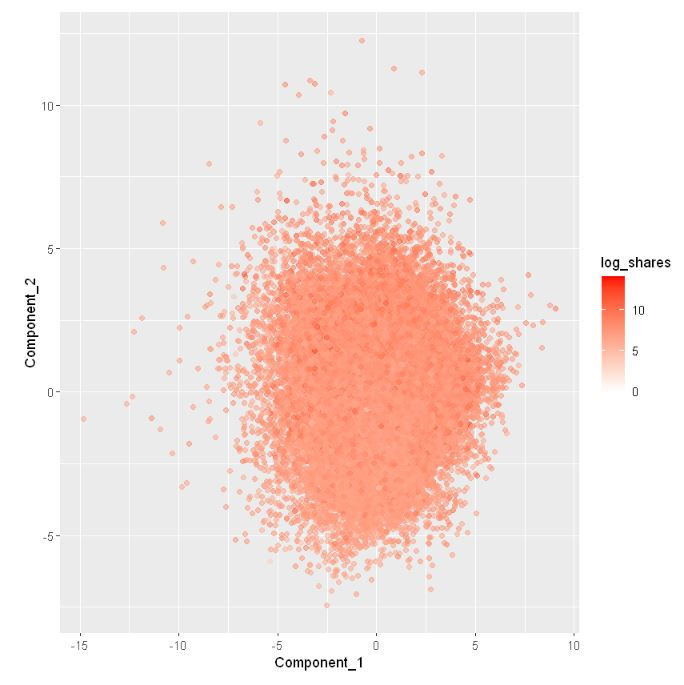
\includegraphics[width=0.4\textwidth]{PCA_12.JPG}
\end{figure}


\begin{figure}[h!]
    \caption{Principal component analysis on 3rd and 4th components}
    \centering
    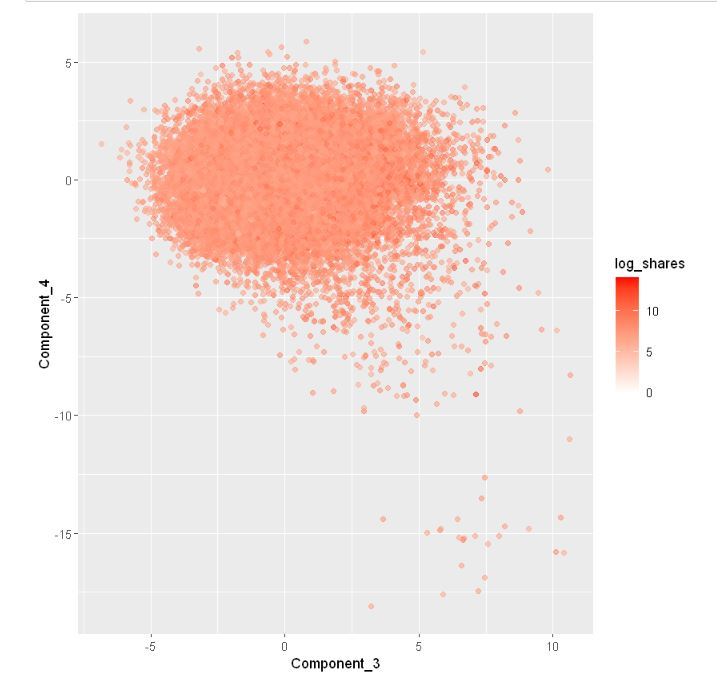
\includegraphics[width=0.4\textwidth]{PCA_34.JPG}
\end{figure}

By the comparing both the figures 3 and 4 ,The variance of the share number is not aligned with the first 4 major components of the variance from independent variables.

\begin{figure}[h!]
    \caption{Heat Map to Check the correlation matrix of the 43 left columns}
    \centering
    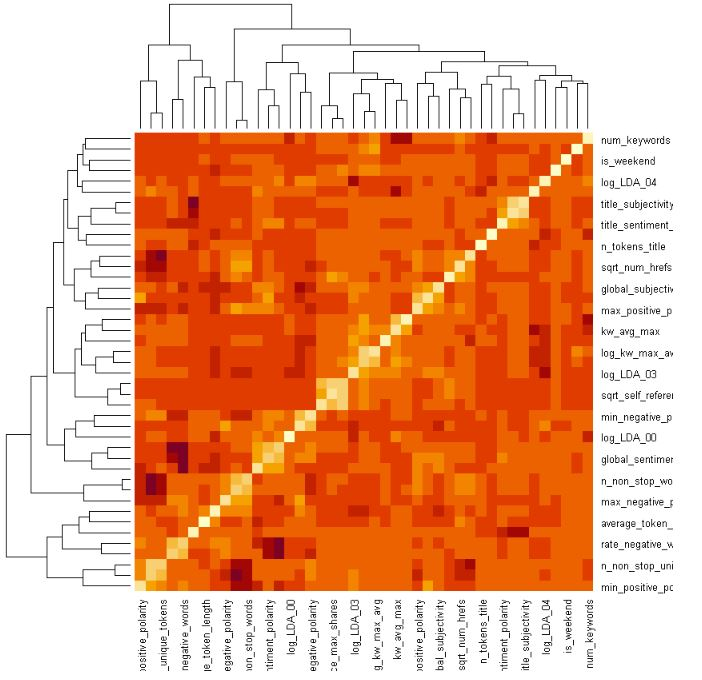
\includegraphics[width=0.5\textwidth]{HeatMap.JPG}
\end{figure}

Lets further look at the correlations of different variables with our dependent variables

\begin{figure}[h!]
    \caption{Correlation of different variables with our dependent variables}
    \centering
    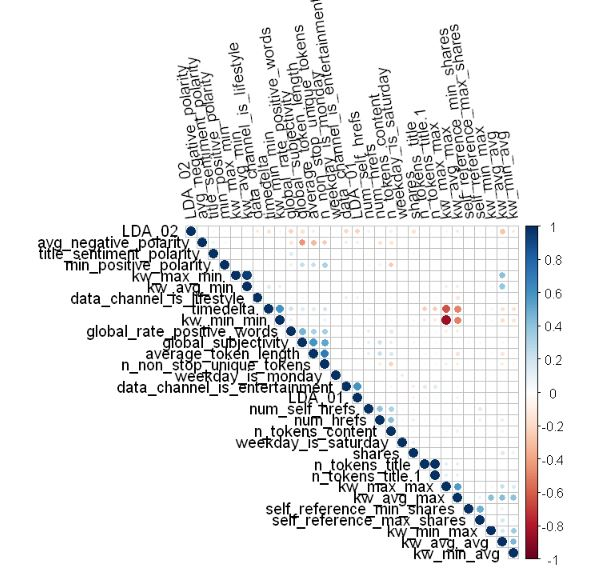
\includegraphics[width=0.5\textwidth]{VisualizingCorelationMatrix.JPG}
\end{figure}

From the heapmap above in Figure 5 ,I can tell there indeed are some groups of variables which are pretty close to each other.
\begin{figure}[h!]
    \caption{Description of the different clusters}
    \centering
    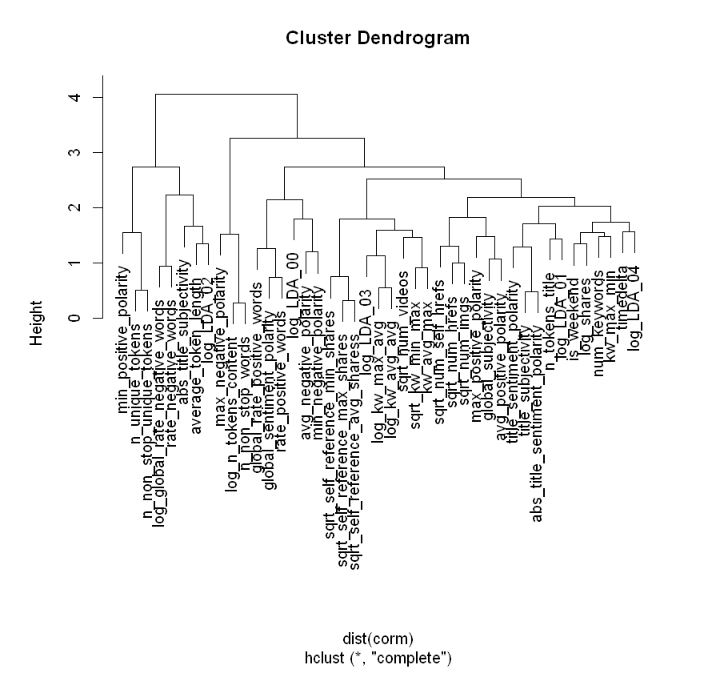
\includegraphics[width=0.5\textwidth]{ClusterDendogram.JPG}
\end{figure}

\section{Modeling}
After preparing the data by removing all the outliers and irrelevant data completely, the dependent variables were identified in the previous section.We start by training different models and identifying the ones that reveal the best accuracy. Before Training the model, it’s important to identify the fact that I have here dealing with a large number of attributes. Thus for effective accuracy I need to train models using algorithms that support large number of attributes. Over considerable tests I have finally shortlisted 4 different algorithms. CART, C50, KNN and Naive Bayes.
\subsection{Regression}
The selected attributes, as listed in the previous section are all numeric. So linear regression model is built to predict the exact value of the target variable. Since the correlation was very mere value the linear regression model couldn’t fit the target value.
For this data is partitioned at 70-30\% for training and testing. The linear model produced the mean R-Square value of 0.02213, which is also very low as compared.
\begin{figure}[h!]
    \caption{Description of the Residuals and Standardized residual over Fitted values}
    \centering
    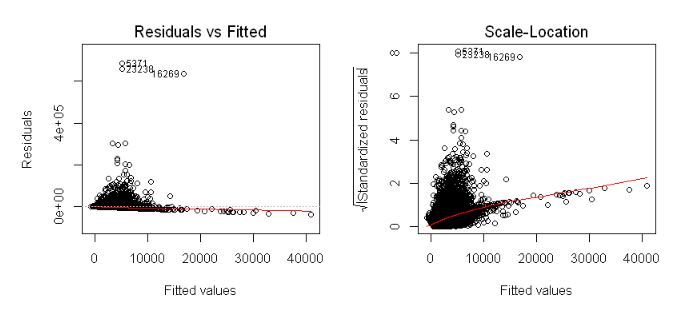
\includegraphics[width=0.45\textwidth]{Regression21.JPG}
\end{figure}
\begin{figure}[h!]
    \caption{Description of the Theoretical Quantiles and Leverage over Standardized residual}
    \centering
    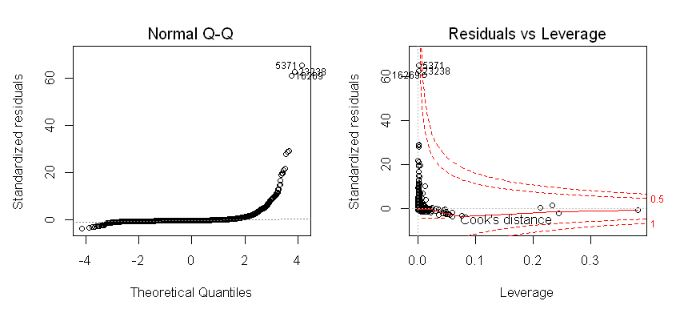
\includegraphics[width=0.45\textwidth]{Regression22.JPG}
\end{figure}


\section{Model Evaluation and Deployment}
\subsection{Naive Bayes Evaluation and Deployment}
I implemented the Naive Bayes model first with a few basic features that I finalised important variables in the data set.
\textbf{First approach:} I used a version of the algorithm that supports numeric attributes and assumes the values of each numerical attribute are normally distributed. This is a strong assumption, but I wanted to check the result.
\begin{figure}[h!]
    \caption{Confusion Matrix of Naive Bayes}
    \centering
    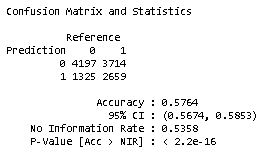
\includegraphics[width=0.50\textwidth]{ConfusionMatrixand Accuracy of NB.JPG}
\end{figure}

I calculated summary stats(mean and standard deviation) of each numerical feature by class values.This of course, gave me a poor accuracy of \textbf{57.64\%} on the validation set.Lets have a look in to the confusion matrix and the ROC details as below
\begin{figure}[h!]
    \caption{ROC of Naive Bayes}
    \centering
    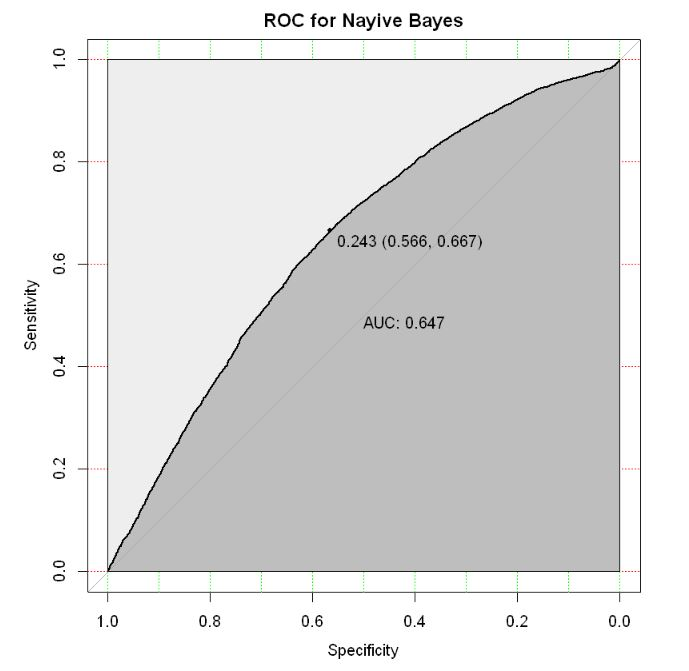
\includegraphics[width=0.50\textwidth]{ROCofNB.JPG}
\end{figure}

\subsection{K-nearest Neighbor-kNN Evaluation and Deployment}
The KNN or k-nearest neighbor algorithm is a type of instance-based learning, where new data are classified based on stored, labeled instances. We work around with different values for k to find the one that best fits our model.Considering several experiments, I have taken k=10.Because it gives best accuracy
\begin{figure}[h!]
    \caption{Confusion Matrix of kNN}
    \centering
    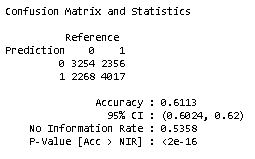
\includegraphics[width=0.50\textwidth]{ConfusionMatrixand Accuracy of kNN.JPG}
\end{figure}

\begin{itemize}
    \item I work around with different values for k to find the one that best fits our model.
    \item Confusion Matrix was developed  to validate the accuracy for every trained Model with best k
\end{itemize}
Displaying the confusion Matrix and ROC Curve for KNN3 as below in Figures
\begin{figure}[h!]
    \caption{ROC of kNN}
    \centering
    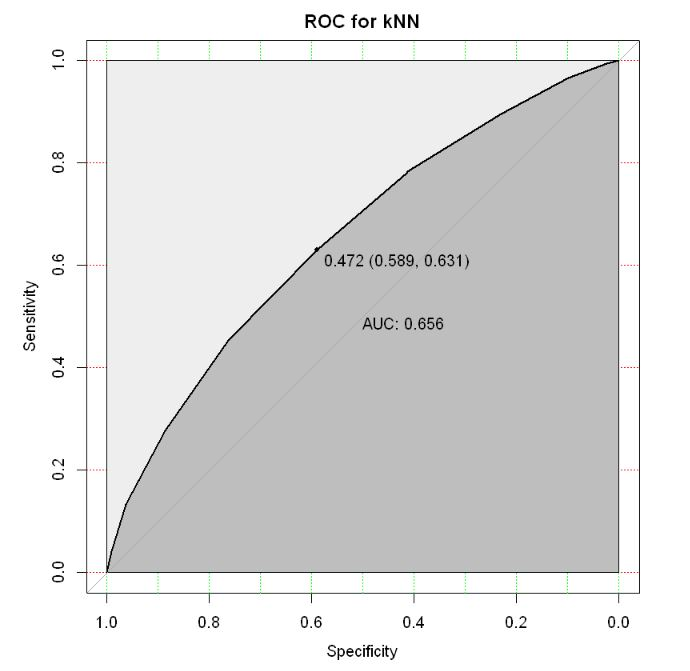
\includegraphics[width=0.50\textwidth]{ROCofKNN.JPG}
\end{figure}


\subsection{Classification and Regression Trees- CART Evaluation and Deployment}

Classification and Regression Trees or CART can be used for logistic regression. The dataset we are working here with requires a better training model than the lazy learning KNN model.

\begin{itemize}
    \item CART forms an intelligent decision tree that improves the overall accuracy of the training model.
    \item Since CART can be used to classify and predict the class label and also to identify any numerical values through Regression
\end{itemize}
\begin{figure}[h!]
    \caption{Confusion Matrix of CART and Accuracy of Model}
    \centering
    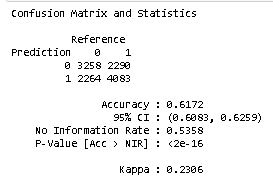
\includegraphics[width=0.50\textwidth]{ConfusionMatrixand Accuracy of CART.JPG}
\end{figure} 

\begin{figure}[h!]
    \caption{ROC of CART}
    \centering
    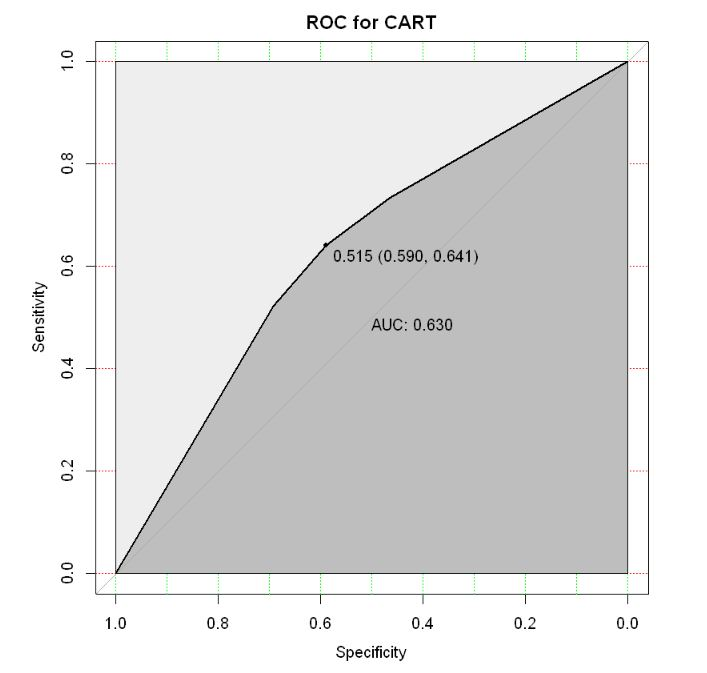
\includegraphics[width=0.50\textwidth]{ROCofCART.JPG}
\end{figure}

\begin{figure}[h!]
    \caption{Decision Trees}
    \centering
    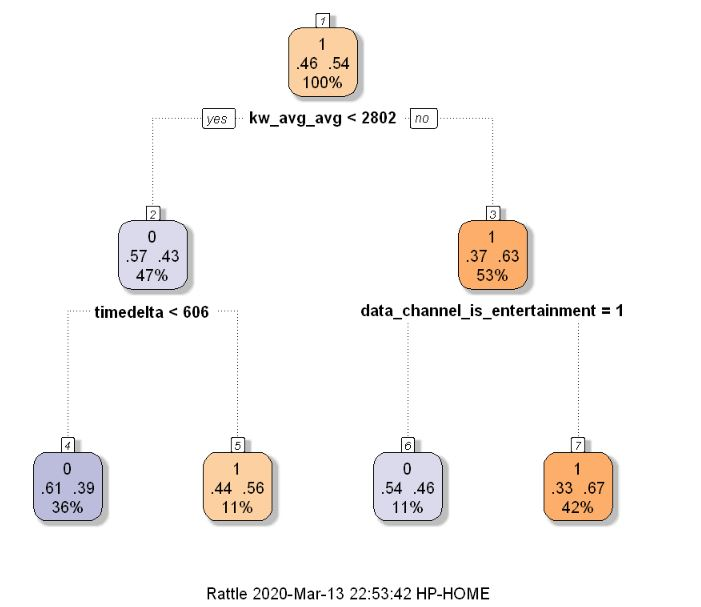
\includegraphics[width=0.50\textwidth]{CART_TREE.JPG}
\end{figure}

\subsection{C.50-Evaluation and Deployment}

So far we have worked on developing training Models using Naive Bayes,KNN and CART methods. The accuracy in either cases has been ordinary. Next we develop a training model using C5.0-Decision Trees. C5.0\cite{PackageC50} is decision trees and rule-based models for Predictions.

\begin{itemize}
    \item C5.0 models are rule based and they work on intelligently retaining the predictions and results as they go over the training data recursively.
    \item The number of trials have an adverse effect on the speed of the training model but with greater trials the accuracy has a marked change.
\end{itemize}

\begin{figure}[h!]
    \caption{Confusion Matrix of C5.0 and Accuracy of Model}
    \centering
    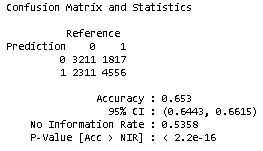
\includegraphics[width=0.50\textwidth]{ConfusionMatrixand Accuracy of C5.0.JPG}
\end{figure} 

\begin{figure}[h!]
    \caption{ROC of C5.0}
    \centering
    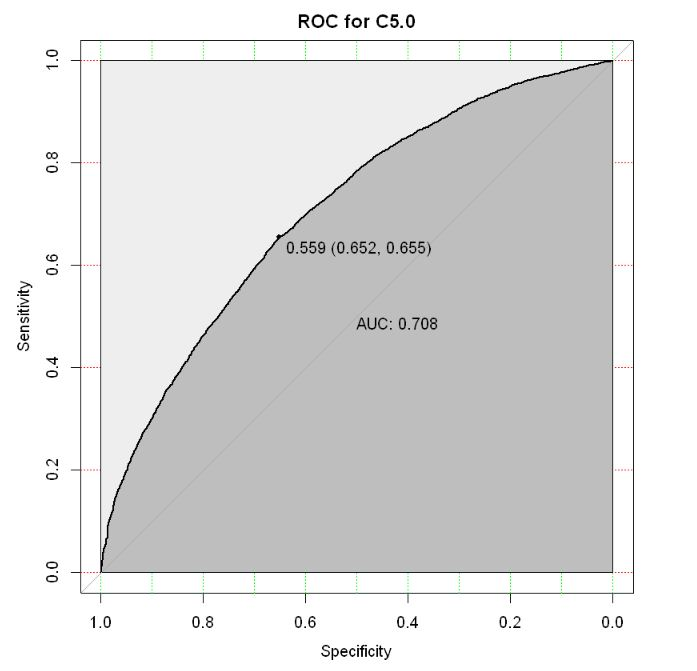
\includegraphics[width=0.50\textwidth]{ROCofC5.0JPG.JPG}
\end{figure}

\section{Conclusion}
The business problem was started with the aim of predicting the reach/popularity of the news article. After multiple levels of cleaning and pre-processing the data is stabilized for model building. Since the linear model couldn’t produce better results because of the variance in the data, various number of bins are used, and classification algorithms are applied. Upon analyzing various models, the suited random forest model is fine tuned.
\begin{itemize}
    \item A comparative study by training different classification models on the dataset and using them to predict output class on testing data has revealed that C5.0 is the best model among all considered models for an accurate prediction of the popularity of an online news article.
    \item Though 2 categories classification provides better and relevant results, it assumes popularity as a definitive output rather than a ranking methodology. In the next steps, instead of categorizing the news article, a ranking mechanism can be built using the bag of words and other text mining, clustering methodologies\cite{Popularity}. 
    \item The ranking methodology can be improved over the period using the reinforcement learning by adding the words from the popular articles to the bag of words normal distribution. In the weighted regression, a more complex fit for the variance could be tried in future work.
\end{itemize}

%%
%% The acknowledgments section is defined using the "acks" environment
%% (and NOT an unnumbered section). This ensures the proper
%% identification of the section in the article metadata, and the
%% consistent spelling of the heading.

%%
%% The next two lines define the bibliography style to be used, and
%% the bibliography file.
\bibliographystyle{ACM-Reference-Format}
\bibliography{DataMiningReportReferences}


\end{document}
\endinput
%%
%% End of file `sample-sigchi.tex'.
